% !TEX root = eds4ltl-paper.tex

\section{Introduction}

Linear temporal logic (LTL) has application to proof of correctness for concurrent programs.
Many concurrent programs, such as operating systems and embedded systems that control physical equipment, are nonterminating by design. 
Consequently, proof techniques that depend on proving the correctness of postconditions on program termination do not apply.
LTL, on the other hand, can be used to prove desirable program traits such as freedom from deadlock.

Linear temporal logic (LTL) has application to proof of correctness for concurrent programs.
Many concurrent programs, such as operating systems and embedded systems that control physical equipment, are nonterminating by design. 
Consequently, proof techniques that depend on proving the correctness of postconditions on program termination do not apply.
LTL, on the other hand, can be used to prove desirable program traits such as freedom from deadlock.

Most treatments of LTL consist of cursory introductions in one or two chapters of graduate-level textbooks. \cite{Baier, Kroger, Manna, Schn}
While many LTL theorems are common in the different treatments, each treatment has theorems that are unique to it.
This survey is a comprehensive collection of all the LTL theorems that we have found in the literature, together with many new theorems, all of which are presented in an axiomatic logic system.
It serves as an introduction to LTL and should be accessible with a prerequisite only of the standard propositional and predicate logic at the undergraduate level.

\subsection{Axiomatic logic systems}

All axiomatic logic systems have three components -- inference rules, axioms, and theorems.
Both inference rules and axioms are assumed.
Theorems are proved from axioms using inference rules.
From a computational systems perspective, the inference rules process axioms as input and produce theorems as output.
Figure \ref{logic-systems} shows the parallel between traditional computational systems and axiomatic logic systems.
In the same way that a processor executes program statements with input to produce output, a proof uses inference rules with axioms to produce theorems.

In a conventional computational system, placement of the hardware/software boundary is a design decision.
Any given computational task can be implemented either in hardware or in software.
The tradeoff in such systems is usually between speed of execution and flexibility.
Usually, a task implemented in hardware executes faster than if it is implemented in software.
However, once implemented in hardware a task is more difficult to modify or extend than if it is implemented in software.
One goal of RISC design is to simplify the hardware by moving tasks from hardware to software.
For example, CISC machines provide complex addressing modes with hardware circuits to compute array cell addresses.
The equivalent address computation is done in software in a RISC machine.

A similar design decision exists in axiomatic logic systems with the placement of the inference rule/axiom boundary.
It is possible to have two different logic systems produce equivalent sets of theorems but with different sets of inference rules and axioms.
What is an inference rule in one system might be a corresponding theorem or axiom in the other.
The tradeoff is more subjective in logic systems, as there is apparently no metric of goodness that can be quantified as objectively as can the speed of execution in computational systems.

This paper presents a logic system that places the boundary between inference rules and axioms to minimize the number of inference rules.
We maintain that the primary advantage of such a system is a human one.
That is, manual proofs in such systems are easier to understand and to design than in other systems.

\begin{figure}[t]
\centering
\begin{picture}(440,46)
\thicklines
\put(0,24) {\fbox{\parbox{36pt}{\centering Input}}}
\put(43,28) {\vector(1,0){20}}
\put(63,24) {\fbox{\parbox{56pt}{\centering Processing}}}
\put(126,28) {\vector(1,0){20}}
\put(146,24) {\fbox{\parbox{42pt}{\centering Output}}}
\put(40,0) {Computational systems}

\put(220,24) {\fbox{\parbox{36pt}{\centering Axioms}}}
\put(263,28) {\vector(1,0){20}}
\put(283,24) {\fbox{\parbox{56pt}{\centering Inference\\rules}}}
\put(346,28) {\vector(1,0){20}}
\put(366,24) {\fbox{\parbox{48pt}{\centering Theorems}}}
\put(250,0) {Axiomatic logic systems}

\end{picture}
\caption{Computational systems and axiomatic logic systems.
\label{logic-systems}}
\end{figure}

\subsection{Propositional logic systems}

Propositional calculus is a formal system of logic based on the unary operator negation $\neg$,
the binary operators conjunction $\land$, disjunction $\lor$, implies $\impl$ (also written $\rightarrow$),
and equivalence $\equiv$ (also written $\leftrightarrow$),
variables (lowercase letters $p$, $q$, \dots), and the constants \textit{true} and \textit{false}.
Hilbert-style logic systems, $\mathcal{H}$, are the deductive logic systems traditionally used in mathematics to describe the propositional calculus.
Typical of such descriptions with applications to computer science is the text by Ben-Ari \cite{Ben}.
A key feature of such systems is their multiplicity of inference rules and the importance of modus ponens as one of them.

In the late 1980's, Dijkstra and Scholten \cite{DandS}, and Feijen \cite{Feij} developed a method of proving program correctness with a new logic based on an equational style.
This equational deductive system, $\mathcal{E}$, is the basis of books by Kaldewaij \cite{Kald} and Cohen \cite{Cohen}.
In contrast to $\mathcal{H}$ systems, $\mathcal{E}$ has only four inference rules -- Substitution, Leibniz, Equanimity, and Transitivity.
In $\mathcal{E}$, modus ponens plays a secondary role.
It is not an inference rule, nor is it assumed as an axiom, but instead is proved as a theorem from the axioms using the inference rules.

Gries and Schneider \cite{Gries1995, Gries1995145} show that $\mathcal{E}$, also known as a \textit{calculational} system, has several advantages over traditional logic systems.
The primary advantage of $\mathcal{E}$ over $\mathcal{H}$ systems is that the equational system has only four proof rules, with inference rule Leibniz as the primary one.
Roughly speaking, Leibniz is ``substituting equals for equals,'' hence the moniker \textit{equational} deductive system.
In contrast, $\mathcal{H}$ systems rely on a more extensive set of inference rules.
We find proofs in $\mathcal{E}$ easy to understand and to teach, because the substitution of equals for equals is common in elementary algebraic manipulations.

Another major advantage of $\mathcal{E}$ over $\mathcal{H}$ systems is the sequential format of its proof syntax.
Proofs in $\mathcal{H}$ systems have a bottom-up tree structure, which is sequentialized with multiple references to previously numbered lines.
For example, a proof of formula $f_2$ might begin by establishing the validity  of a formula $f_1$ on lines 1 through 4.
Then, on lines 5 through 9, it might establish the validity of $f_1\impl f_2$.
Then, on line 10, it would refer back to lines 4 and 9 and invoke modus ponens to establish the validity of $f_2$.

In contrast, proofs in $\mathcal{E}$ have a top-down structure and proceed sequentially with each step self-contained.
There is no need to number the lines in a proof in $\mathcal{E}$ because reference is never made to a previous intermediate step of the proof.
Instead, each line depends only on the immediately preceding line by invoking a previously-proved theorem or an axiom.

There is an analogy between the proof style of $\mathcal{H}$ systems versus the proof style of $\mathcal{E}$ and the unstructured goto style of programming versus structured programming.
In the same way that the goto statement can produce spaghetti code that is more difficult to understand than structured code, proofs in $\mathcal{H}$ systems are more difficult to understand than proofs in $\mathcal{E}$.
It is perhaps not coincidental that Dijkstra, who ignited the goto controversy with his famous CACM letter \cite{Dijkstra:1968:LEG:362929.362947}, was the prime developer of $\mathcal{E}$.

We agree with Gries and Schneider \cite{LADM} that, ``We need a style of logic that can be used as a tool in every-day work.
In our experience, an equational logic, which is based on equality and Leibniz's rule for substitution of equals for equals, is best suited for this purpose.''
These advantages of $\mathcal{E}$ over $\mathcal{H}$ systems are primarily \textit{human} advantages, not necessarily machine advantages.
That is, the motivation behind this work is based on teaching and human understanding, as opposed to machine theorem provers or proof assistants.

In 1994, Gries and Schneider published \textit{A Logical Approach to Discrete Math} (LADM) \cite{LADM}, in which they first develop $\mathcal{E}$ for propositional and predicate calculus, and then extend it to a theory of sets, a theory of sequences, relations and functions, a theory of integers, recurrence relations, modern algebra, and a theory of graphs.
Using equational logic as a tool, LADM brings all the advantages of $\mathcal{E}$ to these additional knowledge domains.
The treatment is in marked contrast to the traditional one exemplified by the classic undergraduate text by Rosen \cite{Rosen}.

\subsection{Linear temporal logic systems}

Linear temporal logic describes how the truth values of propositions change over time.
It extends the propositional operators with the unary operators \textit{next} $\Next$, \textit{eventually} $\Event$, and \textit{always} $\Always$, and the binary operators \textit{until} $\Until$ and \textit{wait} $\Wait$.
Most treatments of linear temporal logic use $\mathcal{H}$ systems instead of $\mathcal{E}$.
Typical are Ben-Ari \cite{Ben2}, Emerson \cite{Emer}, Kröger and Merz \cite{Kroger}, and Manna and Pnueli \cite{Manna}.
Each of these authors describes the semantics of the above temporal operators and provides an axiomatization for linear temporal logic.
One characteristic of these $\mathcal{H}$ systems is the introduction of temporal inference rules along with temporal axioms from which temporal theorems are proved.
Section \ref{comparison-previous-work} summarizes these systems and compares them with this work.

Our institution has used LADM at the introductory undergraduate level since its publication, and the equational proof style has consequently permeated the computer science curriculum.
A problem arises, however, when those who are schooled in $\mathcal{E}$ study concurrency and need the correctness proof tools of linear temporal logic.
Schneider \cite{Schn} appears to be the only treatment of linear temporal logic that uses $\mathcal{E}$.
Although this graduate-level text presents an equational deductive system, the only appearance of an equational proof of a temporal logic theorem is a single example.
Likewise, Baier and Katoen \cite{Baier} have a single equational proof of a linear temporal logic theorem in their chapter on linear temporal logic.

To solve the problem of teaching linear temporal logic at the undergraduate level, this paper presents a comprehensive linear temporal logic system suitable for those versed in the equational deductive system of LADM.
In the same way that LADM brings the advantages of $\mathcal{E}$ to set theory and other mathematical domains, this paper brings the advantages of $\mathcal{E}$ to linear temporal logic.

This axiomatization follows the spirit of $\mathcal{E}$ in its design to minimize the number of inference rules.
A unique characteristic of this system is the complete absence of any temporal inference rules.
It extends the propositional calculus of LADM using only the same four inference rules of $\mathcal{E}$ along with additional temporal axioms.
In our judgment, the absence of temporal inference rules brings the same clarity to linear temporal logic that $\mathcal{E}$ brings to the propositional calculus.

The paper also adds to the linear temporal logic literature by proving many previously unpublished theorems.
It is comprehensive, as we have tried to include all known linear temporal theorems described in the literature.
Although space limitations preclude giving a proof of every theorem in this paper, we have proved every theorem with $\mathcal{E}$.

Section 2 describes the deductive axioms and the proof rules for $\mathcal{E}$.
It also defines the syntax and semantics of linear temporal logic.
Section 3 presents the equational deductive system for linear temporal logic.
Section 4 summarizes previous linear temporal logic axiomatization systems and compares them with the current work.

\section{Background}

The first section below summarizes the equational system $\mathcal{E}$ from LADM \cite{LADM}.
The summary is minimal, and assumes the reader is familiar with the propositional and predicate calculus.
The second section introduces temporal logic and assumes no prior familiarity with it.
The paper can serve as an introduction to linear temporal logic.

\subsection{Equational Deductive Systems}\label{sec-equational-deductive-systems}

\subsubsection{Propositional calculus}

Expressions are the basis of propositional calculus in the equational system.
Propositional theorems are simply boolean expressions that are true in all states.
The definition of an expression has four parts:
\begin{itemize}
\item A constant or variable is an expression.
\item If $E$ is an expression, then $(E)$ is an expression.
\item If $\triangleright$ is a unary prefix operator and $E$ is an expression, then $\triangleright E$ is an expression with operand $E$.
\item If $\star$ is a binary infix operator and $D$ and $E$ are expressions, then $D \star E$ is an expression with operands $D$
and $E$.
\end{itemize}
By convention, upper-case letters ({\itshape e.g.\/} $X$, $Y$, \dots) represent expressions,
and lower-case letters ({\itshape e.g.\/} $x$, $y$, \dots) represent variables.
In the propositional calculus, the constants are {\itshape true\/} and {\itshape false\/}.

Figure \ref{precedence-table} is the table of precedences.
Textual substitution has the highest precedence.
All the unary operators have the next highest precedence.
They are necessarily right associative.
For example, $\neg \Next \neg p$ means $\neg (\Next (\neg p))$.
In this system, two binary operators that have the same precedence require parentheses to disambiguate.
As in LADM, conjunction $\land$ and disjunction $\lor$ have the same precedence so that $p\land q\lor r$
must be disambiguated as either $(p\land q)\lor r$ or $p\land (q\lor r)$.
This contrasts with many systems in which conjunction has higher precedence than disjunction.

\begin{figure}[t]
\centering
%\setlength\extrarowheight{2pt}
\begin{tabular}{lr}
\hline
$[x := e]$ (textual substitution) & Highest precedence\\
$\neg$\quad $\Next$\quad $\Event$\quad $\Always$ &\\
$\Until$\quad $\Wait$ &\\
$=$\quad (conjunctional) &\\
$\lor$\quad $\land$ &\\
$\impl$\quad $\foll$ &\\
$\equiv$ \quad (associative) & Lowest precedence\\
\hline
\end{tabular}
\caption{Precedence of the propositional and temporal logic operators.
\label{precedence-table}}
\end{figure}

Also consistent with the equational system of LADM but different from most other deductive logic systems
is the difference between operators equals $=$ and equivales $\equiv$.
Equals applies to any mathematical type including, {\itshape e.g.\/}, boolean, natural number, and set.
Equivales applies only to boolean, and is commonly denoted $\leftrightarrow$ in other systems.
Another difference is that equals is conjunctive, while equivales is associative.
For example, the expression $p = q = r$ has conjunctive meaning $(p = q) \land (q = r)$, while the expression $p \equiv q \equiv r$
can be taken as either $(p \equiv q) \equiv r$ or $p \equiv (q \equiv r)$.
This property of equivales is the first axiom in the equational deductive system of LADM.

\subsubsection{Inference rules}

The inference rules for the equational deductive system are Substitution, Leibniz, Equanimity, and Transitivity.
\begin{align*}
&\textbf{Substitution:}\quad \frac{E}{E[z:=F]}\\
&\textbf{Leibniz:}\quad \frac{X=Y}{E[z:=X]=E[z:=Y]}\\
&\textbf{Equanimity:}\quad \frac{X, \quad X=Y}{Y}\\
&\textbf{Transitivity:}\quad \frac{X=Y, \quad Y=Z}{X=Z}
\end{align*}
where the square bracket in $E[z:=F]$ indicates textual substitution of expression $F$ for variable $z$
everywhere $z$ occurs in expression $E$.
In a typical proof, Substitution and Leibniz are explicit, while Equanimity and Transitivity are implicit.

Substitution allows the generalization of a single theorem to represent an infinite number of theorems.
For example, because $p\impl \mathit{false} \equiv \lnot p$ is a theorem, then, with $p:=p\land q$, the expression
$(p\land q)\impl \mathit{false} \equiv \lnot (p\land q)$ is also a theorem.

Roughly speaking, Leibniz allows for the substitution of equals for equals in a proof step.
The general form of a proof step is
\begin{tabbing}
\hspace{\mymathindent} \= $= \;$ \=  \kill
  \> \>   $E[z:=X]$\\[\lgap]
  \> $=$  \>  \Hint{$X=Y$} \\[\lgap]
  \> \>   $E[z:=Y]$
\end{tabbing}
where the expression enclosed in angle brackets $\Gll\;\Ggg$, called the ``hint'', is the justification for the step.

An example of a proof step from the proof of theorem (\ref{E:eventAlwaysPAndAlwaysEventQ}) in Section \ref{section-always-continued-2} is
\begin{tabbing}
\hspace{\mymathindent} \= $= \;$ \= \myqedtab \= \kill
\> \>   $\Always (\Always p \land \Event q) \impl \Always\Event (p \land q)$\\[\lgap]
\> $=$  \>  \Hint{(\ref{E:distAlwaysAnd}) Distributivity of $\Always$ over $\land$}\\[\lgap]
\> \>   $\Always \Always p \land \Always\Event q \impl \Always\Event (p \land q)$
\end{tabbing}
This proof step uses the previously proved theorem (\ref{E:distAlwaysAnd}) Distributivity of $\Always$ over $\land$,
which is $\Always (p \land q) \equiv \Always p \land \Always q$.
The justification in the hint $X=Y$ comes from inference rule Substitution, with the textual substitution of $\Always p$ for $p$ and $\Event q$ for $q$ in (\ref{E:distAlwaysAnd}) as follows
\begin{tabbing}
\hspace{\mymathindent} \= $= \;$ \= \myqedtab \= \kill
  \> $(\Always (p \land q) \equiv \Always p \land \Always q)[p,q:=\Always p, \Event q]:\quad \Always (\Always p \land \Event q) \equiv \Always \Always p \land \Always \Event q$
\end{tabbing}
The expressions in Leibniz for the step are
\begin{tabbing}
\hspace{\mymathindent} \= $= \;$ \= \myqedtab \= \kill
  \> $E:\quad z \impl \Always\Event (p \land q)$\\[\lgap]
  \> $X:\quad \Always (\Always p \land \Event q)$\\[\lgap]
  \> $Y:\quad \Always \Always p \land \Always \Event q$
\end{tabbing}
The textual substitutions are
\begin{tabbing}
\hspace{\mymathindent} \= $= \;$ \= \myqedtab \= \kill
  \> $E[z:=X]:\quad \Always (\Always p \land \Event q) \impl \Always\Event (p \land q)$\\[\lgap]
  \> $E[z:=Y]:\quad \Always \Always p \land \Always\Event q \impl \Always\Event (p \land q)$
\end{tabbing}

The proof of a theorem consists of showing the equivalence of that theorem to a previously proved theorem
through a sequence of the proof steps.
For example, here is a one-step proof of (\ref{E:linearity}) $\Next p \equiv \neg\Next\neg p$ in Section \ref{section-next}.

\emph{Proof}:
\begin{tabbing}
\hspace{\mymathindent} \= $= \;$ \= \kill
  \> \>   $\Next p \equiv \neg\Next\neg p$\\[\lgap]
  \> $=$  \>  \Hintfirst{(3.11) $\neg p \equiv q \equiv p \equiv \neg q$ with $p,q := \Next\neg p, \Next p$,} \\[\lgap]
  \> \>   \Hintlast{$\neg \Next\neg p \equiv \Next p \equiv \Next\neg p \equiv \neg \Next p$}\\[\lgap]
  \> \>   $\neg\Next p \equiv \Next\neg p$ \\[\lgap]
  \> which is (\ref{E:selfDual}), Self-dual. \quad \myqed
\end{tabbing}
In a proof hint, numeric references that contain a decimal point, such as (3.11) above, refer to a theorem in $\mathcal{E}$ from LADM.
Equanimity is implicit in the proof.
Because $\neg\Next p \equiv \Next\neg p$ (\textit{i.e.} $X$) is a previous theorem, and $\neg\Next p \equiv \Next\neg p$ is equivalent to $\Next p \equiv \neg\Next\neg p$ (\textit{i.e.} $X=Y$), by equinimity $\Next p \equiv \neg\Next\neg p$ (\textit{i.e.} $Y$) is proved.

Transitivity of equality allows a derivation to be given as a sequence of equivalent expressions, which, at the end,
proves the equivalence of the first expression in the sequence with the last expression in the sequence.
For example, here is a two-step proof of (\ref{E:idemUntil}) Idempotency of $\Until$, $p \Until p \equiv p$ in Section \ref{section-until}.

\emph{Proof}:
\begin{tabbing}
\hspace{\mymathindent} \= $= \;$ \= \myqedtab \= \kill
  \> \>   $p \Until p\equiv p$\\[\lgap]
  \> $=$  \>  \Hint{(\ref{E:expansionUntil}) Expansion of $\Until$}\\[\lgap]
  \> \>   $p \lor (p \land \Next(p \Until p))\equiv p$\\[\lgap]
  \> $=$  \>  \Hint{(3.43b) Absorption, $p \lor (p \land q) \equiv p$ with $q := \Next (p \Until p)$}\\[\lgap]
  \> \>   $p\equiv p$\\[\lgap]
  \> which is (3.5) Reflexivity of $\equiv$. \quad \myqed
\end{tabbing}
Transitivity of equality is implicit in the proof.
Because $p \Until p\equiv p$ is equivalent to $p \lor (p \land \Next(p \Until p))\equiv p$ (\textit{i.e.} $X=Y$),
and $p \lor (p \land \Next(p \Until p))\equiv p$ is equivalent to $p\equiv p$ (\textit{i.e.} $Y=Z$),
by transitivity $p \Until p\equiv p$ is equivalent to $p\equiv p$ (\textit{i.e.} $X=Z$).



% Head 1
\section{MMSN Protocol}

% Head 2
\subsection{Frequency Assignment}

We propose a suboptimal distribution to be used by each node, which is
easy to compute and does not depend on the number of competing
nodes. A natural candidate is an increasing geometric sequence, in
which
% Numbered Equation
\begin{equation}
\label{eqn:01}
P(t)=\frac{b^{\frac{t+1}{T+1}}-b^{\frac{t}{T+1}}}{b-1},
\end{equation}
where $t=0,{\ldots}\,,T$, and $b$ is a number greater than $1$.

In our algorithm, we use the suboptimal approach for simplicity and
generality. We need to make the distribution of the selected back-off
time slice at each node conform to what is shown in
Equation~\eqref{eqn:01}. It is implemented as follows: First, a random
variable $\alpha$ with a uniform distribution within the interval $(0,
1)$ is generated on each node, then time slice $i$ is selected
according to the following equation:
% Unnumbered Equation
\[
i=\lfloor(T+1)\log_b[\alpha(b-1)+1]\rfloor.
\]
It can be easily proven that the distribution of $i$ conforms to Equation
(\ref{eqn:01}).

So protocols \cite{Bahl-02, Culler-01,Zhou-06,Adya-01,
Tzamaloukas-01, Akyildiz-01} that use RTS/CTS
controls\footnote{RTS/CTS controls are required to be implemented by
802.11-compliant devices. They can be used as an optional mechanism
to avoid Hidden Terminal Problems in the 802.11 standard and
protocols based on those similar to \cite{Akyildiz-01} and
\cite{Adya-01}.} for frequency negotiation and reservation are not
suitable for WSN applications, even though they exhibit good
performance in general wireless ad-hoc
networks.

% Head 3
\subsubsection{Exclusive Frequency Assignment}


In exclusive frequency assignment, nodes first exchange their IDs
among two communication hops so that each node knows its two-hop
neighbors' IDs. In the second broadcast, each node beacons all
neighbors' IDs it has collected during the first broadcast period.

% Head 4
\paragraph{Eavesdropping}

Even though the even selection scheme leads to even sharing of
available frequencies among any two-hop neighborhood, it involves a
number of two-hop broadcasts. To reduce the communication cost, we
propose a lightweight eavesdropping scheme.

\subsection{Basic Notations}

As Algorithm 1 states, for each frequency
number, each node calculates a random number (${\textit{Rnd}}_{\alpha}$) for
itself and a random number (${\textit{Rnd}}_{\beta}$) for each of its two-hop
neighbors with the same pseudorandom number generator.

Bus masters are divided into two disjoint sets, $\mathcal{M}_{RT}$
and $\mathcal{M}_{NRT}$.
% description
\begin{description}
\item[RT Masters]
$\mathcal{M}_{RT}=\{ \vec{m}_{1},\dots,\vec{m}_{n}\}$ denotes the
$n$ RT masters issuing real-time constrained requests. To model the
current request issued by an $\vec{m}_{i}$ in $\mathcal{M}_{RT}$,
three parameters---the recurrence time $(r_i)$, the service cycle
$(c_i)$, and the relative deadline $(d_i)$---are used, with their
relationships.
\item[NRT Masters]
$\mathcal{M}_{NRT}=\{ \vec{m}_{n+1},\dots,\vec{m}_{n+m}\}$ is a set
of $m$ masters issuing nonreal-time constrained requests. In our
model, each $\vec{m}_{j}$ in $\mathcal{M}_{NRT}$ needs only one
parameter, the service cycle, to model the current request it
issues.
\end{description}

Here, a question may arise, since each node has a global ID. Why
don't we just map nodes' IDs within two hops into a group of
frequency numbers and assign those numbers to all nodes within two
hops?

\section{Simulator}
\label{sec:sim}

If the model checker requests successors of a state which are not
created yet, the state space uses the simulator to create the
successors on-the-fly. To create successor states the simulator
conducts the following steps.
% enumerate
\begin{enumerate}
\item Load state into microcontroller model.
\item Determine assignments needed for resolving nondeterminism.
\item For each assignment.
      \begin{enumerate}
      \item either call interrupt handler or simulate effect of next instruction, or
      \item evaluate truth values of atomic propositions.
      \end{enumerate}
\item Return resulting states.
\end{enumerate}
Figure~\ref{fig:one} shows a typical microcontroller C program that
controls an automotive power window lift. The program is one of the
programs used in the case study described in Section~\ref{sec:sim}.
At first sight, the programs looks like an ANSI~C program. It
contains function calls, assignments, if clauses, and while loops.
% Figure
\begin{figure}
  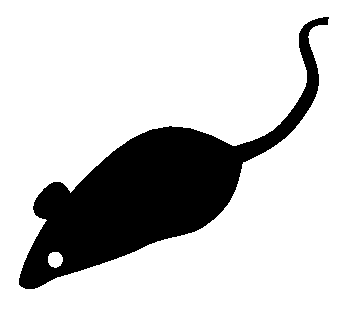
\includegraphics{mouse}
  \caption{Code before preprocessing.}
  \label{fig:one}
\end{figure}

\subsection{Problem Formulation}

The objective of variable coalescence-based offset assignment is to find
both the coalescence scheme and the MWPC on the coalesced graph. We start
with a few definitions and lemmas for variable coalescence.

% Enunciations
\begin{definition}[Coalesced Node (C-Node)]A C-node is a set of
live ranges (webs) in the AG or IG that are coalesced. Nodes within the same
C-node cannot interfere with each other on the IG. Before any coalescing is
done, each live range is a C-node by itself.
\end{definition}

\begin{definition}[C-AG (Coalesced Access Graph)]The C-AG is the access
graph after node coalescence, which is composed of all C-nodes and C-edges.
\end{definition}

\begin{lemma}
The C-MWPC problem is NP-complete.
\end{lemma}
\begin{proof} C-MWPC can be easily reduced to the MWPC problem assuming a
coalescence graph without any edge or a fully connected interference graph.
Therefore, each C-node is an uncoalesced live range after value separation
and C-PC is equivalent to PC. A fully connected interference graph is made
possible when all live ranges interfere with each other. Thus, the C-MWPC
problem is NP-complete.
\end{proof}

\begin{lemma}[Lemma Subhead]The solution to the C-MWPC problem is no
worse than the solution to the MWPC.
\end{lemma}
\begin{proof}
Simply, any solution to the MWPC is also a solution to the
C-MWPC. But some solutions to C-MWPC may not apply to the MWPC (if any
coalescing were made).
\end{proof}

\section{Performance Evaluation}

During all the experiments, the Geographic Forwarding (GF) by Akyildiz
et al.~\shortcite{Akyildiz-01} routing protocol is used. GF exploits
geographic information of nodes and conducts local data-forwarding to
achieve end-to-end routing. Our simulation is configured according to
the settings in Table~\ref{tab:one}. Each run lasts for 2 minutes and
repeated 100 times. For each data value we present in the results, we
also give its 90\% confidence interval.

% Table
\begin{table}%
\caption{Simulation Configuration}
\label{tab:one}
\begin{minipage}{\columnwidth}
\begin{center}
\begin{tabular}{ll}
  \toprule
  TERRAIN\footnote{This is a table footnote. This is a
    table footnote. This is a table footnote.}   & (200m$\times$200m) Square\\
  Node Number     & 289\\
  Node Placement  & Uniform\\
  Application     & Many-to-Many/Gossip CBR Streams\\
  Payload Size    & 32 bytes\\
  Routing Layer   & GF\\
  MAC Layer       & CSMA/MMSN\\
  Radio Layer     & RADIO-ACCNOISE\\
  Radio Bandwidth & 250Kbps\\
  Radio Range     & 20m--45m\\
  \bottomrule
\end{tabular}
\end{center}
\bigskip\centering
\footnotesize\emph{Source:} This is a table
 sourcenote. This is a table sourcenote. This is a table
 sourcenote.

 \emph{Note:} This is a table footnote.
\end{minipage}
\end{table}%


\section{Conclusions}

In this article, we develop the first multifrequency MAC protocol for
WSN applications in which each device adopts a
single radio transceiver. The different MAC design requirements for
WSNs and general wireless ad-hoc networks are
compared, and a complete WSN multifrequency MAC design (MMSN) is
put forth. During the MMSN design, we analyze and evaluate different
choices for frequency assignments and also discuss the nonuniform
back-off algorithms for the slotted media access design.

% Start of "Sample References" section

\section{Typical References in New ACM Reference Format}
A paginated journal article \cite{Abril07}, an enumerated
journal article \cite{Cohen07}, a reference to an entire issue \cite{JCohen96},
a monograph (whole book) \cite{Kosiur01}, a monograph/whole book in a series (see 2a in spec. document)
\cite{Harel79}, a divisible-book such as an anthology or compilation \cite{Editor00}
followed by the same example, however we only output the series if the volume number is given
\cite{Editor00a} (so Editor00a's series should NOT be present since it has no vol. no.),
a chapter in a divisible book \cite{Spector90}, a chapter in a divisible book
in a series \cite{Douglass98}, a multi-volume work as book \cite{Knuth97},
an article in a proceedings (of a conference, symposium, workshop for example)
(paginated proceedings article) \cite{Andler79}, a proceedings article
with all possible elements \cite{Smith10}, an example of an enumerated
proceedings article \cite{VanGundy07},
an informally published work \cite{Harel78}, a doctoral dissertation \cite{Clarkson85},
a master's thesis: \cite{anisi03}, an online document / world wide web
resource \cite{Thornburg01, Ablamowicz07, Poker06}, a video game (Case 1) \cite{Obama08} and (Case 2) \cite{Novak03}
and \cite{Lee05} and (Case 3) a patent \cite{JoeScientist001},
work accepted for publication \cite{rous08}, 'YYYYb'-test for prolific author
\cite{SaeediMEJ10} and \cite{SaeediJETC10}. Other cites might contain
'duplicate' DOI and URLs (some SIAM articles) \cite{Kirschmer:2010:AEI:1958016.1958018}.
Boris / Barbara Beeton: multi-volume works as books
\cite{MR781536} and \cite{MR781537}.

A couple of citations with DOIs: \cite{2004:ITE:1009386.1010128,
  Kirschmer:2010:AEI:1958016.1958018}.

Online citations: \cite{TUGInstmem, Thornburg01, CTANacmart}.

% Appendix
\appendix
\section{Switching Times}

In this appendix, we measure the channel switching time of Micaz
\cite{CROSSBOW} sensor devices.  In our experiments, one mote
alternatingly switches between Channels~11 and~12. Every time after
the node switches to a channel, it sends out a packet immediately and
then changes to a new channel as soon as the transmission is finished.
We measure the number of packets the test mote can send in 10 seconds,
denoted as $N_{1}$. In contrast, we also measure the same value of the
test mote without switching channels, denoted as $N_{2}$. We calculate
the channel-switching time $s$ as
\begin{displaymath}%
s=\frac{10}{N_{1}}-\frac{10}{N_{2}}.
\end{displaymath}%
By repeating the experiments 100 times, we get the average
channel-switching time of Micaz motes: 24.3\,$\mu$s.

\section{Supplementary Materials}


\begin{printonly}
  See the supplementary materials in the online version
\end{printonly}

\begin{screenonly}
\subsection{This is an Example of Appendix Subsection Head}

Channel-switching time is measured as the time length it takes for
motes to successfully switch from one channel to another. This
parameter impacts the maximum network throughput, because motes
cannot receive or send any packet during this period of time, and it
also affects the efficiency of toggle snooping in MMSN, where motes
need to sense through channels rapidly.

By repeating experiments 100 times, we get the average
channel-switching time of Micaz motes: 24.3 $\mu$s. We then conduct
the same experiments with different Micaz motes, as well as
experiments with the transmitter switching from Channel 11 to other
channels. In both scenarios, the channel-switching time does not have
obvious changes. (In our experiments, all values are in the range of
23.6 $\mu$s to 24.9 $\mu$s.)

\subsection{Appendix Subsection Head}

The primary consumer of energy in WSNs is idle listening. The key to
reduce idle listening is executing low duty-cycle on nodes. Two
primary approaches are considered in controlling duty-cycles in the
MAC layer.

\end{screenonly}

\begin{acks}

The authors would like to thank Dr. Maura Turolla of Telecom
Italia for providing specifications about the application scenario.

The work is supported by the \grantsponsor{GS501100001809}{National
  Natural Science Foundation of
  China}{http://dx.doi.org/10.13039/501100001809} under Grant
No.:~\grantnum{GS501100001809}{61273304\_a}
and~\grantnum[http://www.nnsf.cn/youngscientists]{GS501100001809}{Young
  Scientists' Support Program}.


\end{acks}

% Bibliography
\bibliographystyle{ACM-Reference-Format}
\bibliography{sample-bibliography}
